% Provenance (never printed): see sources/outline_sources.md (Year 3: primordial
% nucleosynthesis and stellar burning recalled from the physics books; the s and r
% processes; supernovae and neutron-star mergers; galactic chemical evolution; from the
% solar abundances to the composition of the Earth).
% Brief: sources/book5/BRIEFS.md, ch. 30. Curves from figdata/bachelor-3/
% solar_abundances.py (Asplund, Amarsi and Grevesse 2021, Table 2), neutron_capture.py
% (their Table B.1 isotopes, KADoNiS v0.3 cross sections, IAEA Live Chart half-lives) and
% chemical_evolution.py (closed box against the Geneva-Copenhagen survey of Casagrande et
% al. 2011, and a two-phase [alpha/Fe] model). Exercise and problem values in the Book 5
% scratch calculator calc/ch30.py.
\chapter{元素从何而来}\label{ch:b3:origin-of-elements}

石灰岩悬崖中的钙，绝大部分是在太阳诞生之前
爆发的大质量恒星内部形成的。地核中的铁，大部分
来自另一类爆发，即白矮星的爆发。一枚戒指上的铂，
属于一个丰度峰，该峰由
持续数秒的\omterm{def:b3:origin-of-elements:s-process}{中子俘获}爆发造成，形成于两颗中子星的并合，
或某种罕见的超新星之中；这两者哪一个生成了其中的大部分，
仍有争议。
这些事件都在太阳的成分中留下了印记。太阳的成分，
除行星未能保留的少数元素外，也即太阳系的成分。
本章由此解读这一记录：先给出\omterm{def:b3:origin-of-elements:abundance}{太阳丰度}，
回顾轻元素是如何形成的，
追踪\omterm{def:b3:origin-of-elements:s-process}{中子俘获}如何构造出重元素，
找出各过程发生的场所，并建立模型，说明一个星系的成分
如何随其恒星的生灭而变化。本章末尾回到前几卷地质学的起点：
为什么与太阳由相同物质构成的地球，
铁如此丰富，挥发性元素却如此贫乏。
% ledger: matteucci21:production, cowan21:rprocess, kobayashi20:origins, asplund21:fig1

\begin{recall}
大爆炸核合成、恒星中氢与氦的聚变、
比结合能及其在铁附近的极大值、稳定谷、
β 衰变与半衰期、反应截面、
主序星、红巨星、白矮星、中子星与
超新星等内容均在物理教材中。陨石的分类、CI
球粒陨石、凝聚温度、难熔元素与挥发性
元素、戈尔德施密特分类与全硅酸盐地球，
均见于本科二年级分册中关于行星形成以及
地球中元素的章节。银河系的结构，其薄盘与
\omterm{def:b3:milky-way-galaxies:structure}{厚盘}、晕与\omterm{def:b3:milky-way-galaxies:populations}{星族}，均在
上一章中。
\end{recall}

\section{太阳丰度}\label{sec:b3:origin-of-elements:solar}

太阳占太阳系质量的 \qty{99.85}{\percent} 以上，
其外层保留了太阳系形成之初气体的成分，
但少数轻元素与重元素的缓慢沉降除外。
太阳的成分可由两种途径读取：
一是光球层的吸收线，二是 CI 球粒陨石，
后者是一类陨石，除最易挥发的元素外，
其成分是所有已知物质中与太阳最接近的。
% ledger: asplund21:fig1, asplund21:ci

\begin{definition}[太阳丰度；dex]\label{def:b3:origin-of-elements:abundance}
元素 $X$ 的\emph{太阳丰度}\index{太阳丰度}是
太阳中该元素的原子数与氢原子数之比，
以对数标度表示，氢的对数值取为 $12$：
\[
\log\varepsilon(X) = 12 + \log_{10}\frac{N_X}{N_\mathrm{H}} .
\]
此类对数之差每差一个单位称为一
\emph{dex}\index{dex}：两种丰度相差 $0.3$~dex，即相差
$10^{0.3} \approx 2$ 倍。对恒星而言，其相对于太阳的丰度
用方括号表示，
$[X/\mathrm{H}] = \log_{10}(N_X/N_\mathrm{H})_\star -
\log_{10}(N_X/N_\mathrm{H})_\odot$，同理，对任意两种
元素同样以 $[X/Y]$ 表示。
\end{definition}

下图给出太阳中各元素的丰度，取自一份近期汇编，该汇编重新评估了
全部 83 种长寿元素。铁的 $\log\varepsilon = 7.46$，
即每 \num{34700} 个氢原子对应一个铁原子；
氦则每个氢原子对应 \num{0.0820} 个氦原子。
图中有几处特征十分醒目，本章其余部分将逐一解释。
% ledger: asplund21:abstract, asplund21:ci, data:b5-asplund21

\begin{omfigure}
\centering
\begin{tikzpicture}
\begin{axis}[width=0.95\linewidth, height=8.4cm, xmin=0, xmax=94,
  ymin=-1.8, ymax=12.8, xlabel={原子序数 $Z$},
  ylabel={$\log\varepsilon(X)$ \;($\log\varepsilon(\mathrm{H}) = 12$)},
  tick label style={font=\scriptsize}, label style={font=\small},
  legend style={font=\scriptsize, at={(0.5,-0.17)}, anchor=north,
    legend columns=2, draw=none, cells={anchor=west},
    /tikz/every even column/.append style={column sep=1em}}]
\addplot[blue!70!black, mark=*, mark size=1.3pt, restrict x to domain=0:84]
  table[x=Z, y=logeps] {figdata/out/bachelor-3-solar_abundances-even.dat};
\addlegendentry{偶数 $Z$}
\addplot[blue!70!black, mark=*, mark size=1.3pt, restrict x to domain=88:94, forget plot]
  table[x=Z, y=logeps] {figdata/out/bachelor-3-solar_abundances-even.dat};
\addplot[red!70!black, mark=o, mark size=1.4pt]
  table[x=Z, y=logeps] {figdata/out/bachelor-3-solar_abundances-odd.dat};
\addlegendentry{奇数 $Z$}
\begin{scope}[font=\scriptsize]
\node[anchor=west] at (axis cs:2.2,12.2) {H};
\node[anchor=west] at (axis cs:3.0,10.9) {He};
\node[anchor=west] at (axis cs:5.6,1.0) {Li, Be, B};
\node[anchor=south] at (axis cs:8,8.95) {O};
\node[anchor=south] at (axis cs:6,8.6) {C};
\node[anchor=south, align=center] at (axis cs:26,7.75) {Fe\\[-1pt]峰};
\node[anchor=north] at (axis cs:21,2.95) {Sc};
\node[anchor=south, align=center] at (axis cs:38.5,3.05) {Sr--Zr\\[-1pt]($N = 50$)};
\node[anchor=south] at (axis cs:51.5,2.5) {Te, Xe (r)};
\node[anchor=south, align=center] at (axis cs:58.5,3.7) {Ba\\[-1pt]($N = 82$)};
\node[anchor=south] at (axis cs:76.5,1.95) {Pt (r)};
\node[anchor=south, align=center] at (axis cs:82.5,2.85) {Pb\\[-1pt]($N = 126$)};
\node[anchor=south] at (axis cs:89.6,0.15) {Th};
\node[anchor=north] at (axis cs:92,-0.7) {U};
\end{scope}
\end{axis}
\end{tikzpicture}
\par\smallskip{\small 太阳中各元素的丰度，采用以氢为 12 的对数标度：光球层的观测值，
或对于没有可测光球线的元素，
取 CI 球粒陨石的值，
（Asplund, Amarsi and Grevesse, 2021）。偶数与奇数原子序数分别用两条线绘出。
锝（$Z = 43$）和钷（$Z = 61$）
都没有长寿命同位素，铋与
钍之间的元素亦然。}\label{fig:b3:origin-of-elements:curve}
\end{omfigure}
% ledger: data:b5-asplund21, asplund21:fig1

\begin{enumerate}
\item 氢和氦几乎占了全部原子，
  其数量是其余所有元素之和的一千倍；两者都形成于大爆炸，
  此后又有部分氦在恒星中生成。
\item 锂、铍和硼紧随氦之后，丰度远低于
  碳：铍的丰度低了 1200 万倍。
\item 丰度从氧到重元素急剧下降，
  在氧、铁、钡和铅附近各有一个峰，
  另有若干较小的峰，图中已有标注。
\item 原子序数为偶数的元素比相邻的奇数元素更丰富：
  位于钙和钛之间的钪，比钙约少 \num{1400} 倍，
  比钛约少 \num{68} 倍。这就是
  \emph{奇偶效应}。
\item 过了铁峰之后，曲线趋于平缓：从铁到金，
  丰度下降了 \num{3.5e6} 倍，而从金到铅则
  又回升了十一倍。
\end{enumerate}
% ledger: asplund21:fig1, data:b5-asplund21

按质量计，当前光球层中氢的含量为 $X = 0.7438$，
氦为 $Y = 0.2423$，其余所有元素为 $Z = 0.0139$。若作修正，
则应扣除太阳形成以来已沉降到光球层以下的重元素；
修正后得到原始太阳的值，即太阳诞生时气体的成分，
为 $X = 0.7121$、$Y = 0.2725$ 和 $Z = 0.0154$。
% ledger: asplund21:xyz

\begin{definition}[金属丰度]\label{def:b3:origin-of-elements:metallicity}
恒星或气体的\emph{金属丰度}\index{金属丰度}，是指其中
比氦重的元素含量，天文学中统称为“金属”，
不论其化学性质如何：以质量分数 $Z$ 表示，或
更常用地以相对于太阳的铁丰度 $[\mathrm{Fe/H}]$ 表示。
若某恒星的 $[\mathrm{Fe/H}] = -1$，则其每个氢原子所含的铁
仅为太阳的十分之一。
\end{definition}

\omterm{def:b3:origin-of-elements:abundance}{太阳丰度}的两种来源吻合得非常好。下
图逐元素比较二者。对于 58 种元素，即既不因过于易挥发而在陨石中缺失、
  也未在太阳中被破坏的那些，其
  光球层与 CI 球粒陨石丰度的加权平均差为
$\num[separate-uncertainty=true]{0.000 \pm 0.007}$~\omterm{def:b3:origin-of-elements:abundance}{dex}。两组
数据偏离了这条线。陨石中的氢、氦、
碳、氮、氧和稀有气体远少于太阳：这些元素
在固体凝结时仍留在气体中。太阳所含的锂
比陨石少 \num{200} 倍：它通过核燃烧
破坏了 \qty{99.5}{\percent} 的锂。
% ledger: asplund21:ci, data:b5-asplund21

\begin{omfigure}
\centering
\begin{tikzpicture}
\begin{axis}[width=0.66\linewidth, height=0.66\linewidth, xmin=-3, xmax=12.8,
  ymin=-1, ymax=12.8, xlabel={CI 球粒陨石中的 $\log\varepsilon$},
  ylabel={光球层中的 $\log\varepsilon$},
  tick label style={font=\scriptsize}, label style={font=\small},
  scatter/classes={0={mark=*, mark size=1.3pt, black!70},
    1={mark=square*, mark size=1.5pt, red!70!black},
    2={mark=triangle*, mark size=2pt, blue!70!black}}]
\addplot[black!40, dashed, domain=-1:12.8, samples=2] {x};
\addplot[scatter, only marks, scatter src=explicit symbolic]
  table[x=ci, y=phot, meta=group] {figdata/out/bachelor-3-solar_abundances-compare.dat};
\begin{scope}[font=\scriptsize, red!60!black]
\node[anchor=east] at (axis cs:8.12,12.0) {H};
\node[anchor=west] at (axis cs:1.45,10.914) {He};
\node[anchor=east] at (axis cs:7.25,8.55) {C};
\node[anchor=east] at (axis cs:6.1,7.83) {N};
\node[anchor=west] at (axis cs:8.5,8.45) {O};
\node[anchor=west] at (axis cs:-0.97,8.06) {Ne};
\node[anchor=west] at (axis cs:-0.35,6.38) {Ar};
\node[anchor=west] at (axis cs:-2.12,3.12) {Kr};
\node[anchor=west] at (axis cs:-1.8,2.22) {Xe};
\end{scope}
\node[font=\scriptsize, blue!60!black, anchor=west] at (axis cs:3.4,0.96) {Li};
\end{axis}
\end{tikzpicture}
\par\smallskip{\small 太阳与 CI 球粒陨石的对比：每个点代表
一种元素的两个丰度值（Asplund, Amarsi and Grevesse, 2021；
陨石标度取值使硅吻合）。虚线为相等线。黑点：一致的 58 种元素。
方块：氢、氦、碳、氮、氧和稀有气体，
这些元素未被陨石保留。
三角形：锂，在太阳中
已被破坏。}\label{fig:b3:origin-of-elements:sun-ci}
\end{omfigure}
% ledger: data:b5-asplund21, asplund21:ci

这一吻合对地质学意义重大。它表明：
可在实验室中分析的陨石给出了太阳系的成分，
除最易挥发的元素外；而太阳
的光球层提供氢、碳、氮和氧，补足其余部分。
本科二年级分册正是在这一基础上
建立了整个地球的成分。
% ledger: asplund21:ci

\section{轻元素与恒星}\label{sec:b3:origin-of-elements:stars}

物理学教材描述了大爆炸核合成：在最初的三分钟内，
随着宇宙冷却，质子与中子结合成氘、氦-3、氦-4 以及少量锂-7，
而未生成更重的元素。
观测到的原初丰度为：氦的质量分数
$Y_\mathrm{p} = \num[separate-uncertainty=true]{0.245 \pm 0.003}$，
氘与氢之比为 \num{2.5e-5}，锂与氢之比为
\num{1.45e-10}，后者取自银河系晕中的
老年贫金属恒星。其余所有元素，以及太阳中
多出的氦 $0.2725 - 0.245 \approx 0.028$，都是在恒星中产生的。
% ledger: pdg25:bbn, asplund21:xyz

物理学教材中的恒星在主序上将氢燃烧为氦，
再作为红巨星将氦燃烧为碳和氧；质量最大的恒星
还会在核心周围的壳层中继续燃烧，依次生成氖、镁、
硅，最终生成铁。聚变在铁处停止，因为比结合能
在铁附近最大：通过聚变合成更重的原子核
反而需要吸收能量，而非释放能量。过了铁峰之后，
元素则通过另一条途径形成，即\omterm{def:b3:origin-of-elements:s-process}{中子俘获}，
这是下一节的内容。锂、铍和硼很脆弱：
它们在恒星内部的温度下会被破坏，
这就是太阳几乎耗尽了锂的原因，也是这三种元素
在丰度曲线上形成低谷的原因。

\begin{definition}[α 元素]\label{def:b3:origin-of-elements:alpha}
\emph{α 元素}\index{α 元素}是偶数 $Z$ 的元素之一，即
氧、氖、镁、硅、硫和钙，其最丰富的同位素
（$^{16}\mathrm{O}$、$^{20}\mathrm{Ne}$、
$^{24}\mathrm{Mg}$、$^{28}\mathrm{Si}$、$^{32}\mathrm{S}$、
$^{40}\mathrm{Ca}$）的质量数均为 4 的倍数，
且这些元素主要在大质量恒星中产生，并
通过核心坍缩超新星爆发返回星际气体中。
\end{definition}
% ledger: matteucci21:production, data:b5-asplund21

氧和 \omterm{def:b3:origin-of-elements:alpha}{α 元素}的峰值以及奇偶效应，
都是这些燃烧阶段的标志：氦核并入偶数核，
比并入奇数核更容易，而质子数为偶数的原子核
结合得更紧密。恒星返回气体的
物质取决于其质量。

\begin{definition}[恒星产额]\label{def:b3:origin-of-elements:yield}
由给定初始质量的恒星产生的某元素的\emph{恒星产额}\index{恒星产额}，
是该恒星新生成的该元素的质量，
并以星风及最终爆炸的形式返回星际气体，
占恒星质量的比例。
\end{definition}
% ledger: matteucci21:yield

质量小于 \qty{0.8}{M_\odot} 的恒星寿命长于宇宙的
年龄，且不返回任何物质。质量为 \num{0.8} 至 \qty{8}{M_\odot} 的恒星
通过星风返回氦、氮、碳以及 \omterm{def:b3:origin-of-elements:s-process}{s 过程}的重元素
（钡、钇、锶），最终形成碳–氧
白矮星。质量超过 \num{8} 至 \qty{10}{M_\odot} 的恒星主要产生
\omterm{def:b3:origin-of-elements:alpha}{α 元素}和少量铁，并以核心坍缩
超新星爆发。近距双星中的白矮星可以发生 Ia 型超新星爆发，
这类爆发产生了大部分的铁。
% ledger: matteucci21:production

\begin{omfigure}
\centering
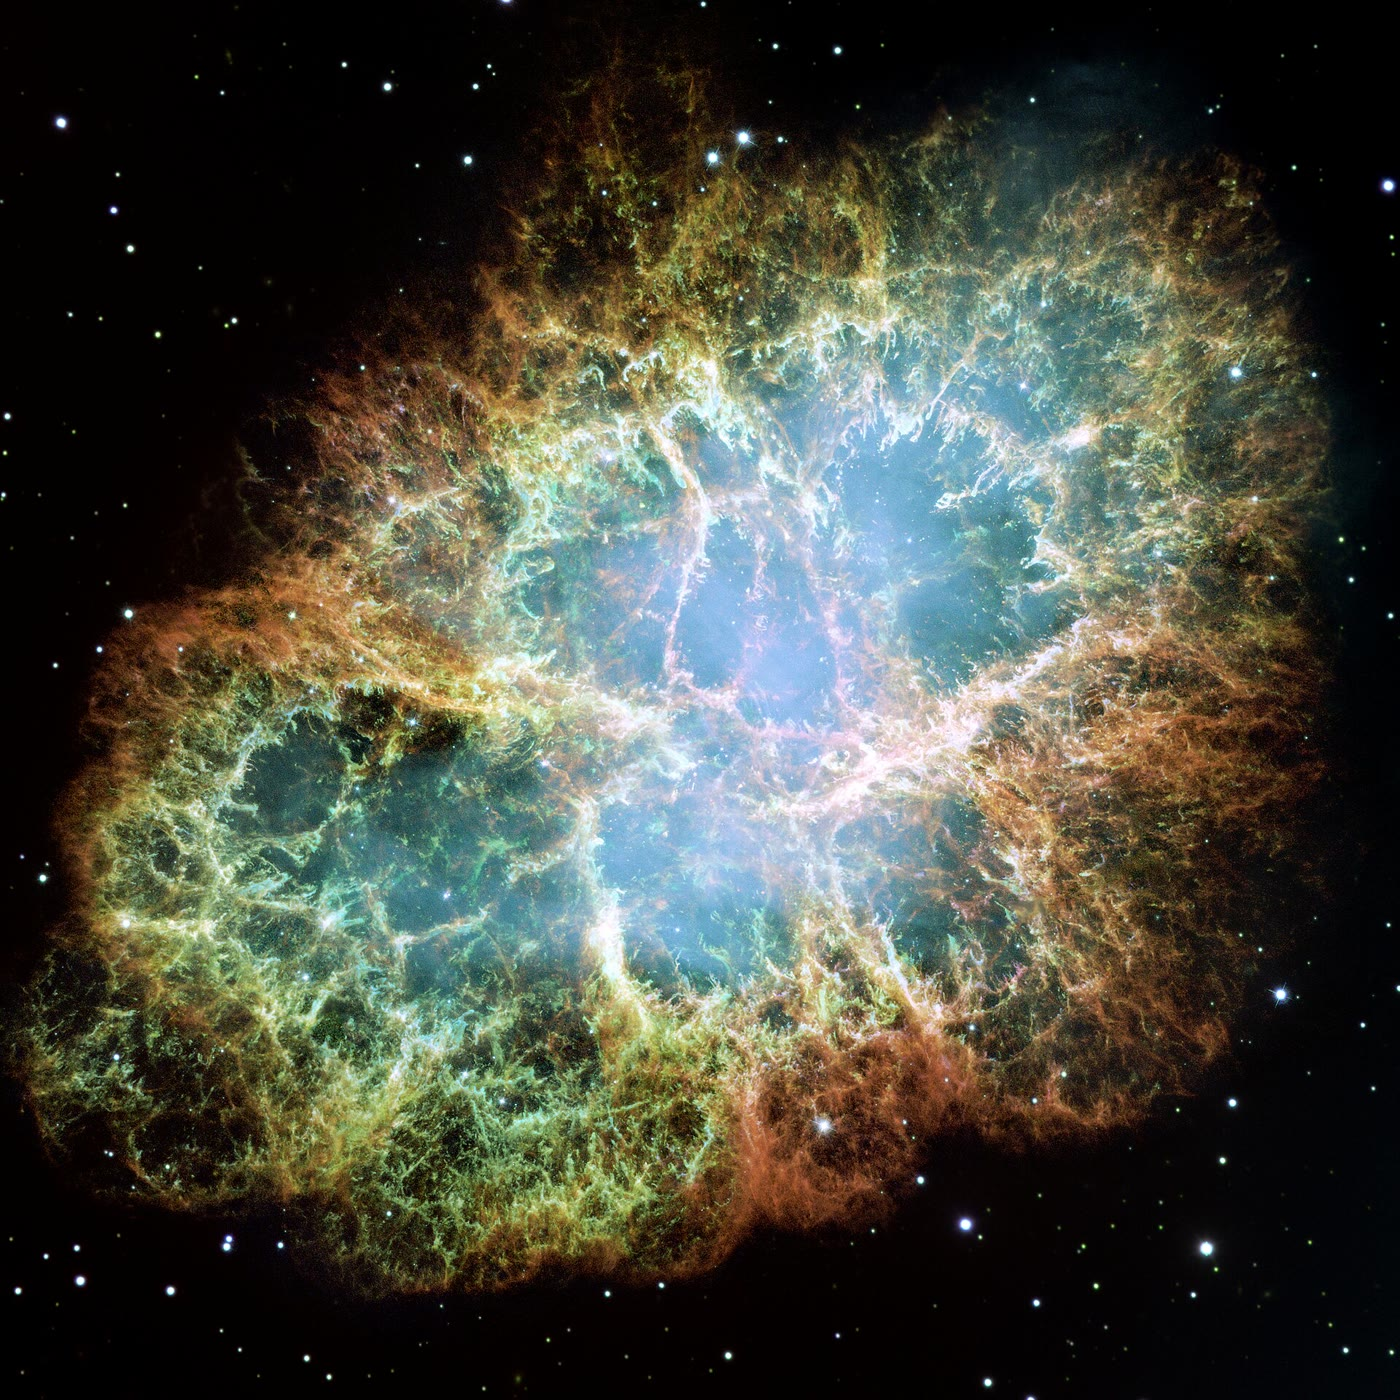
\includegraphics[width=0.5\linewidth]{images/book5/b3-crab-nebula.jpg}
\par\smallskip{\small 蟹状星云，由 24 张哈勃空间望远镜
曝光图像拼接而成，是一颗恒星爆发后膨胀的残余物，其爆发
被日本和中国的天文学家于 1054 年记录下来。橙色的丝状物
是恒星破碎的外层，主要由氢构成；内部发蓝的光
来自电子绕磁感线螺旋运动，这些磁感线属于
位于中心的中子星，该中子星每秒自转 30 次。
丝状气体携带着恒星所合成的物质，
并与星际介质混合。图片来源：NASA、ESA，J.~Hester 和 A.~Loll，公有
领域。}\label{fig:b3:origin-of-elements:crab}
\end{omfigure}
% ledger: photo:b3-crab-nebula

\section{中子俘获}\label{sec:b3:origin-of-elements:neutrons}

中子不带电荷，也不会被原子核排斥：即使是慢中子
也能进入原子核，使原子核质量增加一个质量单位，并
以伽马射线的形式释放结合能。反复俘获会生成
同一元素的更重同位素，直至出现不稳定同位素；它随后
通常经 $\beta^-$ 衰变转变为下一个元素，该元素又依次
俘获中子。生成哪些原子核，取决于一个比较：两次俘获之间的时间
与途中遇到的不稳定原子核的
半衰期之比。

\begin{definition}[中子俘获；s 过程；r 过程]\label{def:b3:origin-of-elements:s-process}
\emph{中子俘获}\index{中子俘获}是原子核吸收一个
自由中子的过程，$(Z, A) + \mathrm{n} \to (Z, A+1) + \gamma$。
在\emph{s 过程}\index{s 过程}（慢）中，俘获
比大多数 β 衰变都慢：同一原子核两次俘获之间的时间
为数百至数千年，因此不稳定核几乎总在
俘获之前衰变，俘获与衰变的链条
沿稳定线进行。在
\emph{r 过程}\index{r 过程}（快）中，中子密度
极高，俘获远快于衰变：原子核
被推向富中子的同位素，远离稳定线，在
数秒内完成，中子耗尽后再衰变回稳定线。
\end{definition}
% ledger: cowan21:timescales, cowan21:rprocess, kaeppeler11:overview

两种过程所达到的原子核不同，
核素图清楚地表明了这一点。下图画出了从镉到
钡的一段。\omterm{def:b3:origin-of-elements:s-process}{s 过程}沿稳定线攀升：沿某元素所在的一行
前进，只要同位素稳定，便继续俘获，再经
一次 β 衰变升到相邻的一行。\omterm{def:b3:origin-of-elements:s-process}{r 过程}来自富中子一侧，位于图的右下方：
每个极度富中子的原子核连续发生 $\beta^-$ 衰变，
沿其同量异位素依次进行，质量数保持不变，直到遇到
第一个稳定核才停止。若某稳定核存在一个稳定的同量异位素，其
$Z$ 更小，则该核被 \omterm{def:b3:origin-of-elements:s-process}{r 过程}\emph{屏蔽}：$^{122}\mathrm{Te}$
位于 $^{122}\mathrm{Sn}$ 之后，$^{123}\mathrm{Te}$ 位于
$^{123}\mathrm{Sb}$ 之后，$^{124}\mathrm{Te}$ 位于 $^{124}\mathrm{Sn}$ 之后。
这三种核只能由 \omterm{def:b3:origin-of-elements:s-process}{s 过程}产生：它们是
\emph{纯 s 核}。反之，$^{128}\mathrm{Te}$ 和 $^{130}\mathrm{Te}$
位于 s 路径之外，s 路径因此止于 $^{127}\mathrm{Te}$，
其半衰期为 \qty{9.35}{h}，它们是纯 r 核。
% ledger: kaeppeler11:overview, data:b5-iaea-gs, data:b5-sigman

\begin{omfigure}
\centering
\begin{tikzpicture}
\begin{axis}[x=0.62cm, y=0.7cm, xmin=61.4, xmax=84.6, ymin=47.4, ymax=56.6,
  xlabel={中子数 $N$}, ylabel={},
  xtick={62,64,...,84}, ytick={48,...,56},
  yticklabels={Cd 48, In 49, Sn 50, Sb 51, Te 52, I 53, Xe 54, Cs 55, Ba 56},
  tick label style={font=\scriptsize}, label style={font=\small},
  axis line style={black!40}, clip=false,
  scatter/classes={0={mark=square*, mark size=6.5pt, blue!45},
    1={mark=square*, mark size=6.5pt, black!18},
    2={mark=square*, mark size=6.5pt, red!40},
    3={mark=square*, mark size=6.5pt, orange!45}}]
\addplot[only marks, mark=square, mark size=6.5pt, black!45, thin,
  restrict x to domain=61:85]
  table[x=N, y=Z] {figdata/out/bachelor-3-neutron_capture-unstable.dat};
\addplot[scatter, only marks, scatter src=explicit symbolic,
  restrict x to domain=61:85]
  table[x=N, y=Z, meta=cls] {figdata/out/bachelor-3-neutron_capture-chart.dat};
\addplot[only marks, mark=none, nodes near coords={\massnum},
  restrict x to domain=61:85,
  visualization depends on={value \thisrow{A} \as \massnum},
  nodes near coords align={center}, every node near coord/.append style={font=\tiny}]
  table[x=N, y=Z] {figdata/out/bachelor-3-neutron_capture-chart.dat};
\addplot[only marks, mark=none, nodes near coords={\massnum}, restrict x to domain=61:85,
  visualization depends on={value \thisrow{A} \as \massnum},
  nodes near coords align={center}, every node near coord/.append style={font=\tiny, black!55}]
  table[x=N, y=Z] {figdata/out/bachelor-3-neutron_capture-unstable.dat};
\addplot[quiver={u=0.48*\thisrow{dN}, v=0.48*\thisrow{dZ}}, -{Stealth[length=3pt]},
  blue!60!black, semithick, restrict x to domain=61:85]
  table[x expr=\thisrow{N0}+0.26*\thisrow{dN}, y expr=\thisrow{Z0}+0.26*\thisrow{dZ}]
  {figdata/out/bachelor-3-neutron_capture-path.dat};
\begin{scope}[red!70!black, dashed, -{Stealth[length=4pt]}, thick]
\draw (axis cs:79.1,48.9) -- (axis cs:76.4,51.6);
\draw (axis cs:81.1,48.9) -- (axis cs:78.4,51.6);
\draw (axis cs:83.1,50.9) -- (axis cs:80.4,53.6);
\end{scope}
\node[font=\scriptsize, red!70!black, anchor=south east, align=right] at (axis cs:84.5,47.5)
  {r 过程衰变 \\[-1pt]沿同量异位素进行};
\end{axis}
\end{tikzpicture}
\par\smallskip{\small 核素图的一段，从镉
到钡，中子数为 62 至 84。有颜色的方块表示自然界中发现的原子核，
标注其质量数：蓝色为纯 s 核，灰色为两种过程均可产生，红色为
纯 r 核，橙色为 \omterm{def:b3:origin-of-elements:p-process}{p 核}，两种过程均无法产生。空心方块为 \omterm{def:b3:origin-of-elements:s-process}{s 过程}
经过的不稳定核。蓝色箭头表示 s 路径：俘获向右进行，
β 衰变斜向左上进行，
（在 $^{134}\mathrm{Cs}$ 和 $^{135}\mathrm{Cs}$ 处路径分叉）。虚线红色
箭头表示三条 \omterm{def:b3:origin-of-elements:s-process}{r 过程}衰变链，分别止于
$^{128}\mathrm{Te}$、$^{130}\mathrm{Te}$ 和 $^{134}\mathrm{Xe}$。
各类别依据自然界中发现的同位素（Asplund、
Amarsi 与 Grevesse，2021）以及 IAEA 核素图中的
半衰期和衰变方式计算得出。}\label{fig:b3:origin-of-elements:chart}
\end{omfigure}
% ledger: data:b5-sigman, data:b5-iaea-gs, data:b5-asplund21, kaeppeler11:branchings

第三组即橙色方块，两种过程都无法到达，
它们是富质子同位素，例如 $^{112}\mathrm{Sn}$、$^{120}\mathrm{Te}$
或 $^{124}\mathrm{Xe}$。

\begin{definition}[p 核]\label{def:b3:origin-of-elements:p-process}
\emph{p 核}\index{p 核}是稳定同位素，位于稳定谷的富质子一侧，
位于铁峰之外，且 \omterm{def:b3:origin-of-elements:s-process}{s 过程}和 \omterm{def:b3:origin-of-elements:s-process}{r 过程}都无法产生它们：
它们被一个原子序数 $Z$ 更小的稳定同量异位素挡住，因而不受 \omterm{def:b3:origin-of-elements:s-process}{r 过程}影响，
且不在 s 路径上。一般认为它们由独立的 p 过程产生，
很可能发生在超新星爆发中，
除少数例外，它们的丰度远小于
相邻的 s 核和 r 核。
\end{definition}
% ledger: kaeppeler11:overview

按照读取核素图的规则，对太阳原始表中锌之后的全部 287 个核素进行判断，
可得 30 个仅由 \omterm{def:b3:origin-of-elements:s-process}{s 过程}产生的核素、29 个仅由 \omterm{def:b3:origin-of-elements:s-process}{r 过程}产生的核素，
以及 36 个 \omterm{def:b3:origin-of-elements:p-process}{p 核}。其中一个 \omterm{def:b3:origin-of-elements:p-process}{p 核} $^{176}\mathrm{Hf}$ 实际上可由 \omterm{def:b3:origin-of-elements:s-process}{s 过程}
经 $^{176}\mathrm{Lu}$ 的一个长寿命激发态产生，简单规则忽略了这一点；
其余 35 个
即文献中的 \omterm{def:b3:origin-of-elements:p-process}{p 核}。
% ledger: data:b5-sigman, kaeppeler11:branchings

\omterm{def:b3:origin-of-elements:s-process}{s 过程}可以定量地加以跟踪，因为其中的核素接近稳定，
其俘获截面可以测量。在温度为 $T$ 的恒星等离子体中，
中子已达到热平衡，因此起作用的是对
麦克斯韦–玻尔兹曼分布取平均的截面 $\langle\sigma\rangle$，
通常在热能
$kT = \qty{30}{keV}$ 下给出。
% ledger: kaeppeler11:classical

\begin{proposition}[$\sigma N$ 关系]\label{prop:b3:origin-of-elements:sigma-n}
\index{sigma N 关系@$\sigma N$ 关系}
在 s 路径的一段上，所有核素都是稳定的，且中子
数密度 $n_\mathrm{n}$ 与温度保持不变。设 $N_A$ 为
质量数为 $A$ 的核素丰度，其平均截面为 $\langle\sigma\rangle_A$。
若中子流已达到稳态，
则
\[
\langle\sigma\rangle_{A-1} N_{A-1} = \langle\sigma\rangle_A N_A ,
\]
因此每个核素的乘积 $\sigma N$
在该段上都相同。
\end{proposition}

\begin{proof}
质量为 $A$ 的核素俘获中子的速率
为 $\lambda_A = n_\mathrm{n}\langle\sigma\rangle_A v_T$（每个核），其中
$v_T$ 为中子的平均热速率。它由
$A - 1$ 核素俘获生成，并因自身的俘获而被消耗，故
$\mathrm{d}N_A/\mathrm{d}t = n_\mathrm{n} v_T\,(\langle\sigma\rangle_{A-1}
N_{A-1} - \langle\sigma\rangle_A N_A)$。在稳态下导数为零，
即得该关系。截面大的核素很快被传递下去，
因而始终稀少；截面小的核素则
会堆积起来。
\end{proof}
% ledger: kaeppeler11:classical

碲的三个仅由 \omterm{def:b3:origin-of-elements:s-process}{s 过程}产生的同位素可以检验这一关系。它们的太阳原始丰度为
\num{0.1067}、\num{0.0373} 和 \num{0.1984}（每百万个硅原子中的原子数），
截面分别为 \num{295}、\num{832} 和
\qty{155}{mb}，乘积分别为 \num{31.5}、\num{31.0} 和
\qty{30.8}{mb}，三者相差不超过 3\%，尽管丰度
相差五倍。跨越中子幻数时该关系失效：
具有 $N = 50$、$82$ 或 $126$ 的核素结合得极紧，
俘获能力很弱，$\langle\sigma\rangle = \qty{4.0}{mb}$ 对应
$^{138}\mathrm{Ba}$，而 $^{136}\mathrm{Ba}$ 为 \qty{61.2}{mb}，
它们起到瓶颈作用。下图给出所有仅由 \omterm{def:b3:origin-of-elements:s-process}{s 过程}产生的核素的乘积，
可见平坦的平台，它们被 $A = 88$、$140$
和 $208$ 附近的台阶隔开。
% ledger: data:b5-sigman, data:b5-kadonis, kaeppeler11:classical

\begin{omfigure}
\centering
\begin{tikzpicture}
\begin{axis}[width=0.95\linewidth, height=7.4cm, xmin=60, xmax=212,
  ymode=log, ymin=1, ymax=5000, xlabel={质量数 $A$},
  ylabel={$\langle\sigma\rangle N$（mb，每 $10^6$ 个 Si 原子）},
  tick label style={font=\scriptsize}, label style={font=\small},
  legend style={font=\scriptsize, at={(0.5,-0.17)}, anchor=north,
    legend columns=2, draw=none, cells={anchor=west},
    /tikz/every even column/.append style={column sep=1em}}]
\draw[black!35, dotted, thick] (axis cs:88,1) -- (axis cs:88,5000);
\draw[black!35, dotted, thick] (axis cs:139,1) -- (axis cs:139,5000);
\draw[black!35, dotted, thick] (axis cs:208,1) -- (axis cs:208,5000);
\addplot[blue!70!black, thick, const plot]
  table[x=A, y=sigN_model] {figdata/out/bachelor-3-neutron_capture-fitted.dat};
\addlegendentry{对 $A > 90$ 拟合的经典模型}
\addplot[only marks, mark=*, mark size=1.7pt, red!70!black]
  table[x=A, y=sigN] {figdata/out/bachelor-3-neutron_capture-sigman.dat};
\addlegendentry{仅 s 过程核素}
\begin{scope}[font=\scriptsize]
\node[anchor=south west] at (axis cs:88.5,1.1) {$N = 50$};
\node[anchor=south west] at (axis cs:139.5,1.1) {$N = 82$};
\node[anchor=south east] at (axis cs:207.5,1.1) {$N = 126$};
\node[anchor=south] at (axis cs:123,38) {Te};
\node[anchor=south] at (axis cs:135,33) {Ba};
\node[anchor=north] at (axis cs:149,6.6) {Sm};
\node[anchor=west] at (axis cs:177,1.79) {Lu};
\node[anchor=west] at (axis cs:71,2326) {Ge};
\node[anchor=west] at (axis cs:83,428) {Kr};
\end{scope}
\end{axis}
\end{tikzpicture}
\par\smallskip{\small 在 \qty{30}{keV} 下的\omterm{def:b3:origin-of-elements:s-process}{中子俘获}截面
（KADoNiS）与太阳原始丰度（Asplund、Amarsi 和 Grevesse，2021）的乘积，
对应 30 个仅由 \omterm{def:b3:origin-of-elements:s-process}{s 过程}产生的核素。在幻数之间（虚线处），
该乘积几乎保持不变，
而在每个幻数处，流动受阻，乘积下降。图中的线是
对 $A = 90$ 以上核素拟合的经典 \omterm{def:b3:origin-of-elements:s-process}{s 过程}模型。
较轻的核素需要第二个较弱的成分，
它产生于大质量恒星中。}\label{fig:b3:origin-of-elements:sigma-n}
\end{omfigure}
% ledger: data:b5-sigman, data:b5-kadonis, data:b5-asplund21, kaeppeler11:classical

图中的线是 \omterm{def:b3:origin-of-elements:s-process}{s 过程}的经典模型：一小部分
$G$ 的铁-56 暴露于中子之中，暴露量围绕均值 $\tau_0$ 呈指数分布，
并沿路径逐核地追踪流量，截面取实测值。该模型对 22 个仅由 \omterm{def:b3:origin-of-elements:s-process}{s 过程}产生的
核素作拟合，这些核素的质量数均大于 $A = 90$
（不计 $^{176}\mathrm{Lu}$（会衰变）、
$^{187}\mathrm{Os}$（由 $^{187}\mathrm{Re}$ 衰变供给）），
拟合得 $\tau_0 = \qty{0.31}{mb^{-1}}$ 和
$G = \qty{0.054}{\percent}$（相对于太阳铁-56），与
\qty{0.04}{\percent} 的详细分析结果接近，在其中每个种子
核平均俘获约十五个中子。最轻的仅由 \omterm{def:b3:origin-of-elements:s-process}{s 过程}产生的
核素锗-70 和硒-76 远高于该线：它们需要
第二个较弱的成分，产生于大质量恒星中。
% ledger: data:b5-sigman, kaeppeler11:classical

当路径上某个不稳定核素的寿命与两次俘获之间的时间
大致相当时，流量发生分支：一部分衰变，另一部分被俘获。
这类\emph{分支}出现在 $^{79}\mathrm{Se}$、$^{85}\mathrm{Kr}$、
$^{134}\mathrm{Cs}$、$^{147}\mathrm{Pm}$ 和 $^{151}\mathrm{Sm}$ 等处，
此外还有其他分支。分支使部分流量绕过某一核素：在两种仅由 \omterm{def:b3:origin-of-elements:s-process}{s 过程}产生的钐同位素中，
$^{150}\mathrm{Sm}$ 接收全部流量，
而 $^{148}\mathrm{Sm}$ 仅接收绕过质量数 147 处分支的那部分流量，
二者的 $\sigma N$ 之比为 \num{0.87}，
由此量度这一份额。由于份额取决于中子密度和
温度，分支便是
\omterm{def:b3:origin-of-elements:s-process}{s 过程}发生处恒星的温度计和密度计。
% ledger: kaeppeler11:branchings, kaeppeler11:pairs, data:b5-sigman

\begin{inthelab}[测量俘获截面]
为测量 \omterm{def:b3:origin-of-elements:s-process}{s 过程}所需的平均截面，
物理学家在加速器上再现恒星中子能谱。
质子轰击锂靶，通过反应
$^{7}\mathrm{Li}(\mathrm{p},\mathrm{n})^{7}\mathrm{Be}$ 产生中子，其能谱
模拟 $kT = \qty{25}{keV}$ 的热分布，接近
红巨星氦壳闪的 \qty{23}{keV}。样品紧贴靶放置，
处于最强通量处。辐照之后，
对新生成的放射性核素所发出的伽马射线进行计数：
这种活化法可用于质量不足一微克的样品。
若产物稳定，则以脉冲形式发出中子，
并沿飞行路径计时以确定其能量。样品周围的一个
氟化钡晶体球记录每次俘获的伽马射线
级联。
\end{inthelab}
% ledger: kaeppeler11:lab

\begin{history}[红巨星中的锝]
1952 年，梅里尔在
光谱型为 S 的红巨星光谱中找到了锝的谱线。锝没有稳定同位素；
由 \omterm{def:b3:origin-of-elements:s-process}{s 过程}产生的 $^{99}\mathrm{Tc}$ 半衰期为
\num{211000} 年，远短于这些恒星
已经历的寿命。锝必然是在恒星内部生成的，且是近期的。
这是恒星制造元素的第一个直接证据。
1957 年，伯比奇夫妇、福勒和霍伊尔，
以及独立工作的卡梅伦，
提出了 \omterm{def:b3:origin-of-elements:s-process}{s 过程}的经典模型。
\end{history}
% ledger: kaeppeler11:overview, data:b5-iaea-gs

\omterm{def:b3:origin-of-elements:s-process}{r 过程}也留下了自己的峰。其路径紧贴中子滴线，
即超过该线后核素便无法再束缚另一个中子的界限，
流量会在中子壳层闭合的核素处停滞，即 $N = 50$、$82$ 和
$126$，直至发生 β 衰变。这些等待点堆积物质；
经最终衰变至稳定后，这些堆积位于比同一幻数的 \omterm{def:b3:origin-of-elements:s-process}{s 过程}峰
低数个单位的质量数处，
后者由稳定核素构成：$A = 130$ 附近的碲和氙，以及
$A = 195$ 附近的铂，而 \omterm{def:b3:origin-of-elements:s-process}{s 过程}峰对应的是 $A = 138$ 和 $208$，
即钡和铅。丰度曲线并列显示两组峰，
\omterm{def:b3:origin-of-elements:s-process}{r 过程}生成约一半的重元素，\omterm{def:b3:origin-of-elements:s-process}{s 过程}
生成另一半。
% ledger: cowan21:rprocess, kaeppeler11:overview, kaeppeler11:classical

\section{过程发生的场所}\label{sec:b3:origin-of-elements:sites}

\omterm{def:b3:origin-of-elements:s-process}{s 过程}的主要部分发生在质量不超过约三个太阳质量的红巨星中，
处于其生命末期，作为渐近巨星支恒星。在核心周围壳层中的氦燃烧闪之间，
形成一层富含碳-13 的薄层，
在约 \qty{9e7}{K} 时，反应
$^{13}\mathrm{C}(\alpha,\mathrm{n})^{16}\mathrm{O}$ 释放中子，
持续约一万年，中子密度为 $10^6$ 至
\num{e8}\text{ 个中子}\,\unit{cm^{-3}}。闪光本身期间，温度高于
\qty{2.5e8}{K} 时，$^{22}\mathrm{Ne}(\alpha,\mathrm{n})^{25}\mathrm{Mg}$
产生持续数年、中子密度可达 \qty{e10}{cm^{-3}} 的爆发。产物
被翻卷至表面，在那里可观测到锝，
并被恒星风吹散。弱 \omterm{def:b3:origin-of-elements:s-process}{s 过程}负责生成质量数小于 $A = 90$ 的
仅由 \omterm{def:b3:origin-of-elements:s-process}{s 过程}产生的核素，它发生在大质量恒星的氦燃烧与
碳燃烧阶段。
% ledger: kaeppeler11:sources, kaeppeler11:overview

核心坍缩型超新星是质量超过八至十个太阳质量的恒星的终结，
它们在恒星诞生后不久释放出 \omterm{def:b3:origin-of-elements:alpha}{α 元素}和一部分铁，
原因是大质量恒星寿命很短。Ia 型超新星，
即在双星中爆炸的白矮星，释放出大部分
铁，但需经过一段延迟：白矮星须先由
质量不足八个太阳质量的恒星形成，之后或从伴星吸积物质，
直至达到钱德拉塞卡质量，约
\qty{1.44}{M_\odot}，或与第二颗白矮星并合。\omterm{def:b3:origin-of-elements:s-process}{r 过程}需要更为极端的
环境。
% ledger: matteucci21:production, matteucci21:time-delay

\begin{definition}[中子星并合；千新星]\label{def:b3:origin-of-elements:kilonova}
\emph{中子星并合}\index{中子星并合}是指近距双星中两颗中子星的
合并，其轨道因引力波辐射而收缩。
富含中子的物质中有一部分被抛射出去。
\emph{千新星}\index{千新星}是这些抛射物的瞬变光辉，
由新合成的 \omterm{def:b3:origin-of-elements:s-process}{r 过程}核素的放射性衰变加热，
持续数天。
\end{definition}
% ledger: cowan21:kilonova, ligo17:gw170817

2017 年 8 月 17 日，引力波探测器记录到
两颗中子星螺旋靠近的过程 GW170817，距离约为
\qty{40}{Mpc}：两个天体的质量分别为 \num{1.17} 至 \qty{1.60}{M_\odot}，合计
\qty{2.74}{M_\odot}。伽马射线暴在并合后 \qty{1.7}{s} 抵达。
不到十一小时后，望远镜在星系 NGC~4993 中发现了一个新的光点
（见下图）。其紫外辉光在两天内减弱，
十天内其光变为红色并转向红外。
该演化的模型需要数种抛射物成分，其中最红的一种
富含镧系元素，即较重的 \omterm{def:b3:origin-of-elements:s-process}{r 过程}元素，其致密的
谱线“密林”使抛射物不透明。抛射物总质量估计为
\num{0.03} 至 \qty{0.08}{M_\odot}：
\omterm{def:b3:origin-of-elements:kilonova}{中子星并合}产生 \omterm{def:b3:origin-of-elements:s-process}{r 过程}元素的首个直接证据。
% ledger: ligo17:gw170817, mma17:kilonova, cowan21:kilonova

\begin{omfigure}
\centering
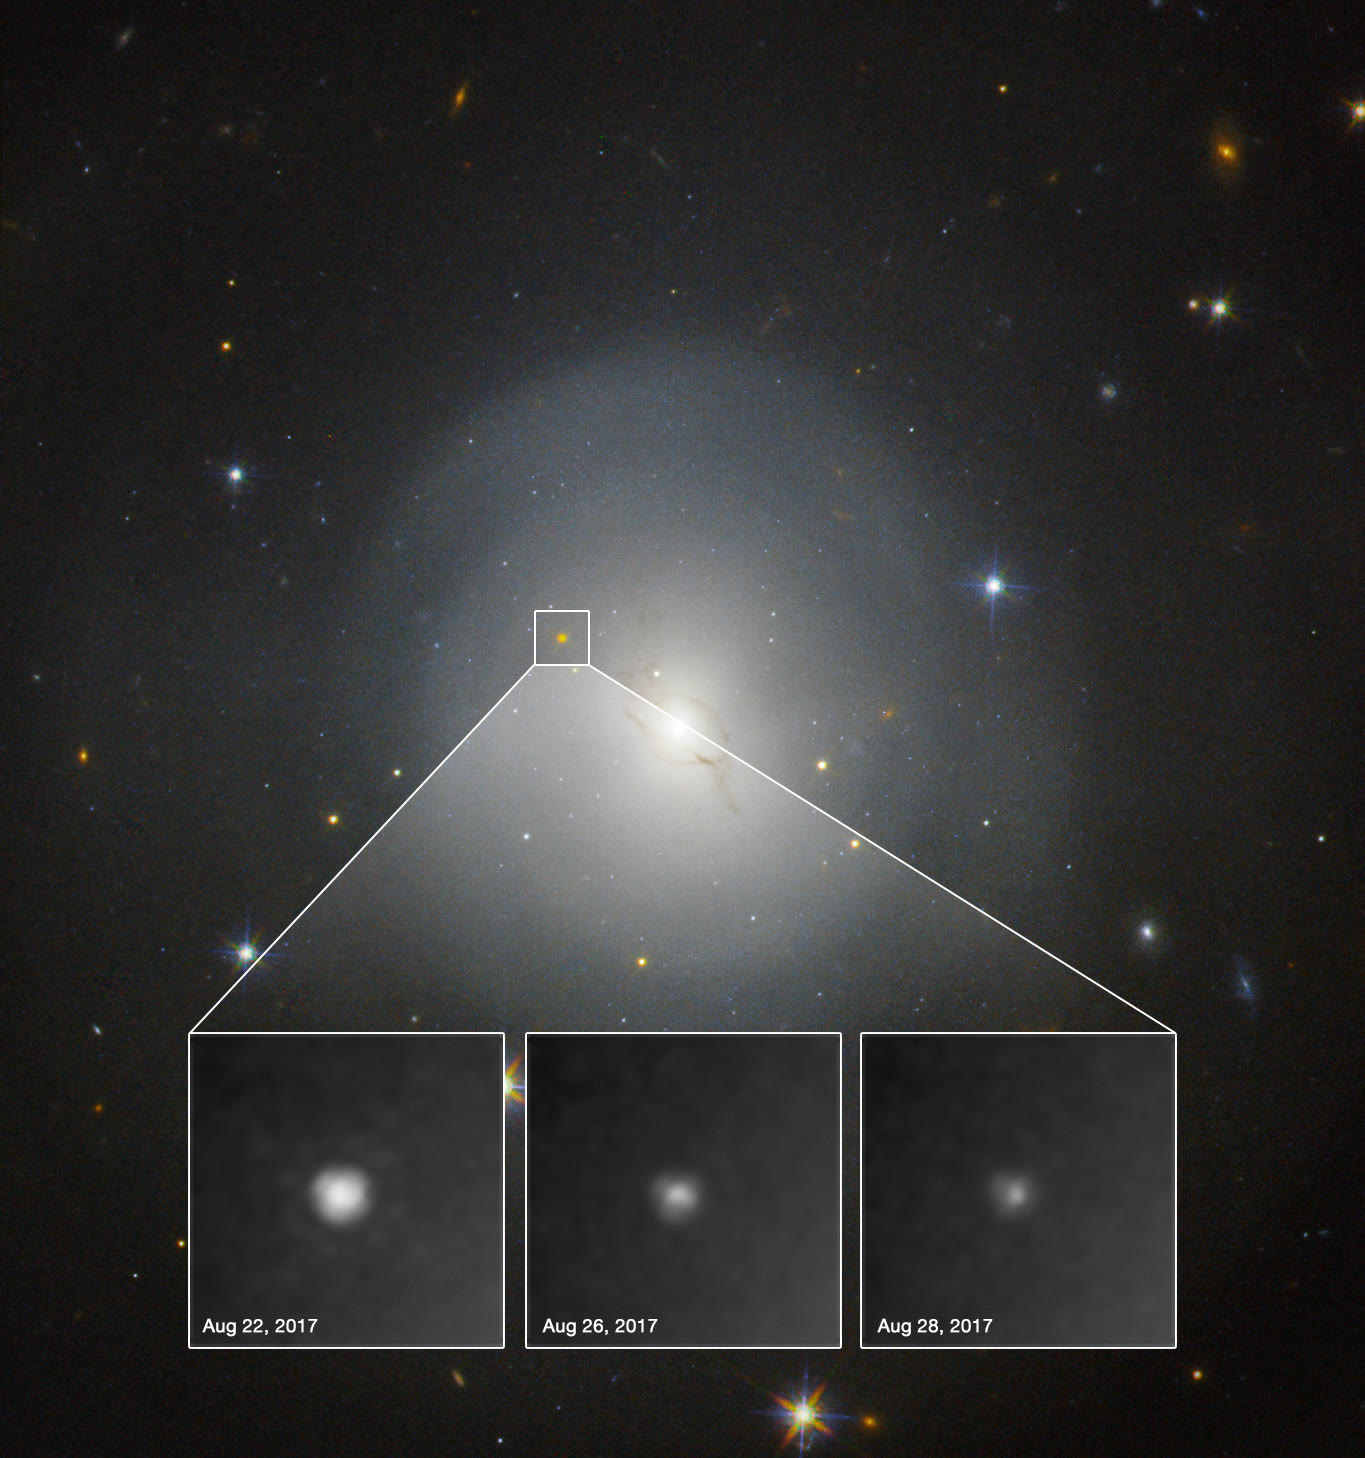
\includegraphics[width=0.55\linewidth]{images/book5/b3-kilonova.jpg}
\par\smallskip{\small 星系 NGC~4993，由哈勃
太空望远镜拍摄，摄于两颗\omterm{def:b3:origin-of-elements:kilonova}{中子星并合}之后。
这两颗中子星于 2017 年 8 月 17 日经引力波探测到，方框标出\omterm{def:b3:origin-of-elements:kilonova}{千新星}；
插图拍摄于 8 月 22、26 和 28 日，显示其在六天内逐渐变暗。
NASA 与 ESA（A.~J.~Levan、N.~R.~Tanvir、A.~Fruchter 和 O.~Fox），CC
BY~4.0。}\label{fig:b3:origin-of-elements:kilonova}
\end{omfigure}
% ledger: photo:b3-kilonova

\begin{dated}{2021}
\omterm{def:b3:origin-of-elements:kilonova}{中子星并合}是否产生了银河系中大部分的 \omterm{def:b3:origin-of-elements:s-process}{r 过程}
元素，尚无定论。并合须等待双星轨道衰减，
若银河系演化模型中并合是唯一来源，
则 \omterm{def:b3:origin-of-elements:s-process}{r 过程}元素出现得过晚，无法解释所见的
最古老、\omterm{def:b3:origin-of-elements:metallicity}{金属丰度}最低的恒星。罕见的核心坍缩超新星，
自转快速、磁场强大，以及极大质量恒星的坍缩，
也是其他候选者；一个银河系模型
能解释观测到的铕丰度，前提是约 3\% 的
质量为 25 至 \qty{50}{M_\odot} 的极超新星属于磁驱动
类型。
\end{dated}
% ledger: kobayashi20:origins, cowan21:rprocess

\section{银河系的化学演化}\label{sec:b3:origin-of-elements:gce}

每一代恒星都会把自身合成的一部分物质归还给气体，
下一代恒星便由这种富集的气体形成。因此，恒星的成分
记录了它诞生时气体的成分，而
同一星系中按年龄排列的恒星，记录了该星系的历史。

\begin{definition}[银河系化学演化]\label{def:b3:origin-of-elements:gce}
\emph{银河系化学演化}\index{银河系化学演化}
是指星系中气体和恒星的成分
随时间的变化，由恒星形成、\omterm{def:b3:origin-of-elements:yield}{恒星产额}、
恒星寿命，以及流入或流出星系的气体共同作用所致；
而对这一变化的研究，是借助
模型与已知年龄恒星丰度的比较进行的。
\end{definition}
% ledger: matteucci21:simple

最简单的模型把星系中的一个区域视为一个混合充分的气体箱，
气体缓慢转化为恒星。设 $s$ 为锁定在
长寿恒星与恒星遗迹中的质量，$M_\mathrm{g}$ 为
气体的质量，$M = M_\mathrm{g} + s$ 为总质量。\emph{每代\omterm{def:b3:origin-of-elements:yield}{恒星产额}}
$y$ 指一代恒星每锁定单位质量，
归还给气体的新金属质量。
% ledger: matteucci21:yield

\begin{theorem}[闭箱模型]\label{thm:b3:origin-of-elements:closed-box}
\index{闭箱模型}
考虑一个与外界不交换气体、起始为
不含金属的纯气体、始终充分混合的区域，其中产金属的恒星
立即死亡，其余恒星永远存在（瞬时
回收）。于是，气体的\omterm{def:b3:origin-of-elements:metallicity}{金属丰度}为
\[
Z = y \ln\frac{1}{\mu}, \qquad \mu = \frac{M_\mathrm{g}}{M},
\]
其中 $\mu$ 为气体份额，\omterm{def:b3:origin-of-elements:metallicity}{金属丰度}低于 $Z$ 的恒星
质量为 \mbox{$M\,(1 - \mathrm{e}^{-Z/y})$}。
\end{theorem}

\begin{proof}
当质量 $\mathrm{d}s$ 被锁定进恒星时，气体失去 $\mathrm{d}s$，
连同其中的金属 $Z\,\mathrm{d}s$，
并获得 $y\,\mathrm{d}s$ 的新金属：
即 $\mathrm{d}M_\mathrm{g} = -\mathrm{d}s$，且
$\mathrm{d}(Z M_\mathrm{g}) = (y - Z)\,\mathrm{d}s$。将第二式
展开，得 $M_\mathrm{g}\,\mathrm{d}Z + Z\,\mathrm{d}M_\mathrm{g} =
y\,\mathrm{d}s - Z\,\mathrm{d}s$，其中含 $Z$ 的项相消：
$M_\mathrm{g}\,\mathrm{d}Z = -y\,\mathrm{d}M_\mathrm{g}$。积分
由 $M_\mathrm{g} = M$、$Z = 0$ 出发，得 $Z = y\ln(M/M_\mathrm{g})$。
\omterm{def:b3:origin-of-elements:metallicity}{金属丰度}低于 $Z$ 时形成的恒星，是在
气体从 $M$ 降至 $M\mathrm{e}^{-Z/y}$ 期间形成的，其质量为
$M(1 - \mathrm{e}^{-Z/y})$。
\end{proof}
% ledger: matteucci21:simple

该模型预言了长寿恒星的\omterm{def:b3:origin-of-elements:metallicity}{金属丰度}分布。
在太阳邻域中，气体的面密度为
\qty{13.7}{M_\odot.pc^{-2}}，恒星与恒星遗迹的面密度为
\qty{33.4}{M_\odot.pc^{-2}}，故 $\mu = 13.7/47.1 = 0.29$。若今天的气体
具有原太阳的 $Z = 0.0154$，则产额为
$y = 0.0154/\ln(1/0.29) = 0.0125$，且迄今形成的全部恒星中，
\omterm{def:b3:origin-of-elements:metallicity}{金属丰度} $Z$ 低于当前值十分之一的比例
（若铁随金属变化，即 $[\mathrm{Fe/H}] < -1$）为
$(1 - 0.29^{0.1})/(1 - 0.29) = 0.16$。
% ledger: mckee15:surface, asplund21:xyz, data:b5-gce

\begin{omfigure}
\centering
\begin{tikzpicture}
\begin{axis}[width=0.95\linewidth, height=7.2cm, xmin=-1.6, xmax=0.7,
  ymin=0, ymax=1500, xlabel={$[\mathrm{Fe/H}]$},
  ylabel={恒星数（每 \num{0.1}~dex）},
  tick label style={font=\scriptsize}, label style={font=\small},
  legend style={font=\scriptsize, at={(0.5,-0.17)}, anchor=north,
    legend columns=3, draw=none, cells={anchor=west},
    /tikz/every even column/.append style={column sep=1em}}]
\addplot[ybar, area legend, bar width=0.085, fill=black!25, draw=black!50, bar shift=0pt]
  table[x=feh, y=n_obs] {figdata/out/bachelor-3-chemical_evolution-mdf.dat};
\addlegendentry{F 型与 G 型矮星（6670）}
\addplot[ybar, area legend, bar width=0.085, fill=blue!55, draw=blue!70!black, bar shift=0pt]
  table[x=feh, y=n_low] {figdata/out/bachelor-3-chemical_evolution-mdf.dat};
\addlegendentry{质量不超过 \qty{1}{M_\odot}（902）}
\addplot[red!75!black, very thick, const plot mark mid]
  table[x=feh, y=model] {figdata/out/bachelor-3-chemical_evolution-mdf.dat};
\addlegendentry{闭箱模型}
\draw[black!50, dashed] (axis cs:-1,0) -- (axis cs:-1,1500);
\node[font=\scriptsize, anchor=north west, align=left] at (axis cs:-1.57,1450)
  {闭箱模型：\qty{16}{\percent}\\低于 $-1$；\\观测值：\qty{0.4}{\percent}};
\end{axis}
\end{tikzpicture}
\par\smallskip{\small \omterm{def:b3:origin-of-elements:g-dwarf}{G 矮星问题}。柱状图：太阳邻域的 F 型与 G 型矮星的\omterm{def:b3:origin-of-elements:metallicity}{金属丰度}
（Geneva--Copenhagen
巡天，最佳测光样本经 Casagrande 等人重新分析，
2011 年），全部恒星为灰色；质量不超过一个太阳质量的，即模型所计入的
长寿恒星为蓝色。折线为\omterm{thm:b3:origin-of-elements:closed-box}{闭箱
模型}，取太阳邻域当前的气体份额，并缩放到
相同恒星数；该模型不产生比当前气体更富金属的恒星，
当前气体取为太阳值。\omterm{thm:b3:origin-of-elements:closed-box}{闭箱模型}预言了一条长长的贫金属
恒星尾，而这一尾部实际并不存在。}\label{fig:b3:origin-of-elements:g-dwarf}
\end{omfigure}
% ledger: data:b5-gcs, casagrande11:gcs, data:b5-gce, mckee15:surface

\begin{definition}[G 矮星问题]\label{def:b3:origin-of-elements:g-dwarf}
\emph{G 矮星问题}\index{G 矮星问题}是指太阳邻域中
贫金属长寿恒星相对于\omterm{thm:b3:origin-of-elements:closed-box}{闭箱模型}预测数目的短缺：
光谱型为 G 的长寿矮星中，\omterm{def:b3:origin-of-elements:metallicity}{金属丰度}低的
远少于\omterm{thm:b3:origin-of-elements:closed-box}{闭箱
模型}所能产生的数量。
\end{definition}
% ledger: matteucci21:simple

在巡天样本的 6670 颗恒星中，有 26 颗的 $[\mathrm{Fe/H}] < -1$：
占 \qty{0.4}{\percent}，而\omterm{thm:b3:origin-of-elements:closed-box}{闭箱模型}的这一比例为 \qty{16}{\percent}。
即便只看质量不超过一个太阳质量的 902 颗恒星，
这是最公平的比较，其中 26 颗占 \qty{2.9}{\percent}。摆脱困境的办法是打开
闭箱：若太阳邻域的\omterm{def:b3:milky-way-galaxies:structure}{银盘}由缓慢流入的贫金属气体构成，
历经数十亿年逐步形成，则早期气体
从来不是一个等待生成贫金属恒星的大储库，因而
这一尾部便消失了。能够再现该分布的\omterm{def:b3:milky-way-galaxies:structure}{银盘}模型需要
超过三十亿至四十亿年的流入时间。
% ledger: data:b5-gcs, data:b5-gce, matteucci21:simple

第二个“时钟”是两类元素的比值。
\omterm{def:b3:origin-of-elements:alpha}{α 元素}来自核心坍缩超新星，在一个恒星
世代诞生后不久即产生；大部分铁则来自 Ia 型超新星，
发生得要晚得多。在 $[\mathrm{Fe/H}] < -1$ 的老晕族恒星中，
$[\alpha/\mathrm{Fe}]$ 约为 $+0.4$：这些恒星由
仅经核心坍缩超新星富集的气体形成。在\omterm{def:b3:milky-way-galaxies:structure}{银盘}恒星中，它随
\omterm{def:b3:origin-of-elements:metallicity}{金属丰度}升高而降至零，即太阳值，随着 Ia 型超新星
贡献其铁。下图给出这一
\emph{时间延迟}图景的最简单模型：在闭箱中，两类超新星同时开始，
只是 Ia 型超新星总在最早的恒星出现之后
经过一段固定的延迟才开始。
% ledger: matteucci21:time-delay, matteucci21:production

\begin{omfigure}
\centering
\begin{tikzpicture}
\begin{axis}[width=0.8\linewidth, height=6.4cm, xmin=-2.4, xmax=0.25,
  ymin=-0.08, ymax=0.55, xlabel={$[\mathrm{Fe/H}]$},
  ylabel={$[\alpha/\mathrm{Fe}]$},
  tick label style={font=\scriptsize}, label style={font=\small}]
\addplot[black!40, dashed, domain=-2.4:0.25, samples=2] {0};
\addplot[blue!70!black, very thick]
  table[x=feh, y=afe] {figdata/out/bachelor-3-chemical_evolution-alpha.dat};
\addplot[only marks, mark=*, mark size=2pt, red!70!black] coordinates {(-1,0.4) (0,0)};
\node[font=\scriptsize, anchor=south, align=center] at (axis cs:-1.75,0.41)
  {仅核心坍缩超新星};
\node[font=\scriptsize, anchor=south west, align=left] at (axis cs:-0.98,0.41)
  {Ia 型超新星 \\[-1pt]开始};
\node[font=\scriptsize, anchor=south west] at (axis cs:0.01,0.01) {太阳};
\end{axis}
\end{tikzpicture}
\par\smallskip{\small 闭箱中 $[\alpha/\mathrm{Fe}]$ 的两阶段模型：
平台位于 $+0.4$，为核心坍缩超新星所产生的比值；
Ia 型超新星在气体达到
$[\mathrm{Fe/H}] = -1$ 时开始出现，此后以稳定速率添加铁，
直至 $[\mathrm{Fe/H}] = 0$ 处比值为太阳值。平台与膝
是银河系恒星中所见的特征，中间的形状则是模型的。
在太阳\omterm{def:b3:origin-of-elements:metallicity}{金属丰度}处，该模型中 \qty{60}{\percent} 的铁
来自 Ia 型超新星。}\label{fig:b3:origin-of-elements:alpha}
\end{omfigure}
% ledger: data:b5-gce, matteucci21:time-delay

再现观测趋势的银河系详细模型
取三分之二的铁来自 Ia 型超新星，三分之一来自
核心坍缩超新星，并发现年轻银河系的气体达到
$[\mathrm{Fe/H}] = -1$ 的时间约在十亿至十五亿年之间。
这一比值是一个“时钟”：在给定\omterm{def:b3:origin-of-elements:metallicity}{金属丰度}下 \omterm{def:b3:origin-of-elements:alpha}{α 元素}丰富的\omterm{def:b3:milky-way-galaxies:populations}{星族}，
其恒星形成得很快，早在 Ia 型超新星
能够添加其铁之前。上一章的\omterm{def:b3:milky-way-galaxies:structure}{厚盘}便是这样一个\omterm{def:b3:milky-way-galaxies:populations}{星族}：
年代古老，与相同\omterm{def:b3:origin-of-elements:metallicity}{金属丰度}的薄盘恒星相比，
\omterm{def:b3:origin-of-elements:alpha}{α 元素}略为富集。
% ledger: matteucci21:time-delay, casagrande11:gcs

\section{从太阳丰度到地球}\label{sec:b3:origin-of-elements:earth}

地球由与太阳相同的物质构成，但并非全部。
在冷却的星云中，只有凝结成固体的元素
才能聚集成星子；本科二年级分册依照其凝结次序
展开讨论。铁以金属形式凝结，其凝结温度与
镁硅酸盐大致相同，约为 \qtyrange{1310}{1340}{K}，
在 \qty{e-4}{bar} 下，因此岩质行星保留了其中的铁，而
氢、氦、碳、氮及稀有气体则留在气体中。
在太阳组成的气体中，仅约百分之零点五的质量
会凝结为岩石与金属。
% ledger: lodders:tc-table, lodders:condensates

\begin{definition}[挥发性趋势]\label{def:b3:origin-of-elements:volatility}
行星天体的\emph{挥发性趋势}\index{挥发性趋势}是指其丰度
相对于 CI 球粒陨石、以难熔元素归一化后，
随凝结温度降低而下降的程度：难熔元素保持其
球粒陨石中的比例，中等挥发性元素则
凝结温度越低，
亏损越严重。
\end{definition}

对于硅酸盐地球，本科二年级分册给出了
随凝结温度变化的趋势。以镁归一化，
锆（凝结温度 \qty{1741}{K}）为其 CI 比例的 \num{1.11} 倍，钠
（\qty{958}{K}）为 \num{0.22}，钾（\qty{1006}{K}）为
\num{0.19}，铷（\qty{800}{K}）为 \num{0.12}，
锌（\qty{726}{K}）为 \num{0.075}。地球由
已在行星组装之前失去部分中等挥发性元素的物质
形成，或在生长过程中失去了这些元素。即便是 CI 球粒陨石，
与太阳的差异遵循凝结温度的规律，
只是程度较轻：其中等挥发性元素的丰度
比光球值约高 \num{0.04}~\omterm{def:b3:origin-of-elements:abundance}{dex}。
% ledger: lodders:tc-table, lodders:ci-table, ms95:pm-trace, asplund21:abstract

因此，本章的线索贯穿整个行星。地幔中的氧、
镁和硅是来自大质量恒星的 \omterm{def:b3:origin-of-elements:alpha}{α 元素}；
地核中的铁主要来自 Ia 型超新星；
钍和铀的衰变有助于加热内部，它们位于铋之外，
只有 \omterm{def:b3:origin-of-elements:s-process}{r 过程}才能到达那里；而整个混合物
在地球聚集它之前已按挥发性完成分选。
% ledger: matteucci21:production, matteucci21:time-delay, kaeppeler11:overview, data:b5-sigman

\section{练习}

\begin{exercise}[$\star$]\label{exo:b3:origin-of-elements:1}
利用\omterm{def:b3:origin-of-elements:abundance}{太阳丰度} $\log\varepsilon(\mathrm{O}) = 8.69$，
$\log\varepsilon(\mathrm{Si}) = 7.51$，$\log\varepsilon(\mathrm{Fe}) =
7.46$，$\log\varepsilon(\mathrm{Au}) = 0.91$ 以及
$\log\varepsilon(\mathrm{Pb}) = 1.95$：(a)~太阳中每个铁原子对应多少个硅原子，
以及多少个氧原子？(b)~每个金原子对应多少个铁原子，
以及多少个铅原子？
\end{exercise}

\begin{exercise}[$\star$]\label{exo:b3:origin-of-elements:2}
(a)~太阳中每一百万个氢原子含有多少个铁原子
（$\log\varepsilon(\mathrm{Fe}) = 7.46$）？(b)~一颗晕星的
$[\mathrm{Fe/H}] = -2$，它每个铁原子对应多少个氢原子？
(c)~另一颗恒星每一千万个氢原子含有一个铁原子，
它的 $[\mathrm{Fe/H}]$ 是多少？
\end{exercise}

\begin{exercise}[$\star$]\label{exo:b3:origin-of-elements:3}
氙的稳定同位素质量数分别为 124、126、128、129、130、
131、132、134 和 136。在它们的同量异位素中，碲（$Z = 52$）的稳定同位素
质量数为 120、122--126、128 和 130；碘（$Z = 53$）只有 127。
\omterm{def:b3:origin-of-elements:s-process}{s 过程}路径在 $^{128}\mathrm{Xe}$ 处到达氙，经
$^{128}\mathrm{I}$ 衰变而来，并在 $^{133}\mathrm{Xe}$ 处离开该路径，后者会衰变。
将每个氙同位素分类：仅由 \omterm{def:b3:origin-of-elements:s-process}{s 过程}产生、仅由 \omterm{def:b3:origin-of-elements:s-process}{r 过程}产生、
由两者共同产生，或为 \omterm{def:b3:origin-of-elements:p-process}{p 核}。
\end{exercise}

\begin{exercise}[$\star$]\label{exo:b3:origin-of-elements:4}
GW170817 位于约 \qty{40}{Mpc} 处，其伽马射线
在引力波所见的并合之后 \qty{1.7}{s} 才到达。(a)~两种信号
各自传播了多长时间？
(b)~若将这一延迟完全归因于两者速度之差，该差值
至多占光速的多大比例？
\end{exercise}

\begin{exercise}[$\star\star$]\label{exo:b3:origin-of-elements:5}
碲的三种仅由 \omterm{def:b3:origin-of-elements:s-process}{s 过程}产生的同位素，其原始\omterm{def:b3:origin-of-elements:abundance}{太阳丰度}分别为
\num{0.1067}、\num{0.0373} 和 \num{0.1984}（每 $10^6$ 个硅原子）
（$A = 122$、$123$、$124$），其平均截面分别为 \num{295}、
\num{832} 和 \qty{155}{mb}。(a)~分别计算各同位素的 $\sigma N$。(b)~仅依据
$^{122}\mathrm{Te}$ 的数据，预测 $^{123}\mathrm{Te}$
和 $^{124}\mathrm{Te}$ 的丰度，并加以比较。(c)~为何该关系
不能用于 $^{128}\mathrm{Te}$？
\end{exercise}

\begin{exercise}[$\star\star$]\label{exo:b3:origin-of-elements:6}
在经典模型中，\omterm{def:b3:origin-of-elements:s-process}{s 过程}路径上的每个原子核都会
将流量中比例为 $f = 1/(1 + 1/(\tau_0\langle\sigma\rangle))$ 的部分传给下一个原子核，
其中 $\tau_0 = \qty{0.306}{mb^{-1}}$。(a)~计算下列核的 $f$：
$^{124}\mathrm{Te}$（\qty{155}{mb}）及中子幻数核
$^{138}\mathrm{Ba}$（\qty{4.0}{mb}）的值。(b)~\omterm{def:b3:origin-of-elements:s-process}{s 过程}路径上从
$^{137}\mathrm{Ba}$ 到 $^{142}\mathrm{Nd}$ 的各原子核，其截面依次为
\num{76.3}、\num{4.0}、\num{32.4}、\num{11.0}、
\num{111.4} 和 \qty{35.0}{mb}。求 $\sigma N$ 从
$^{136}\mathrm{Ba}$ 到 $^{142}\mathrm{Nd}$ 下降了多少倍？(c)~将结果
与测量值 \num{27.6} 和 \qty{7.72}{mb} 相比较。
\end{exercise}

\begin{exercise}[$\star\star$]\label{exo:b3:origin-of-elements:7}
热能为 $kT$ 的中子，其速度为
$v_T = \sqrt{2kT/m_\mathrm{n}}$，$m_\mathrm{n} = \qty{1.6749e-27}{kg}$。
(a)~计算 $v_T$，其中 $kT = \qty{8}{keV}$ 为红巨星
中碳-13 层的温度。(b)~对 $^{124}\mathrm{Te}$，
$\langle\sigma\rangle = \qty{155}{mb}$，计算两次俘获之间的平均时间
$1/(n_\mathrm{n}\langle\sigma\rangle v_T)$，分别取
$n_\mathrm{n} = 10^6$、$10^8$ 和 \qty{e10}{cm^{-3}}。(c)~将其与
$^{127}\mathrm{Te}$（\qty{9.35}{h}）的半衰期和
$^{134}\mathrm{Cs}$（\qty{2.07}{\text{年}}）的半衰期相比较，哪一个是分支点？
\end{exercise}

\begin{exercise}[$\star\star$]\label{exo:b3:origin-of-elements:8}
在太阳中，钙的 $\log\varepsilon$ 为 \num{6.30}，钪为
\num{3.14}，钛为 \num{4.97}；铍为 \num{1.38}，
硼为 \num{2.70}，碳为 \num{8.46}。(a)~钪比其两个相邻元素
少多少倍？(b)~铍比碳少多少倍？
(c)~每项分别说明丰度曲线的哪一特征，
其成因是什么？
\end{exercise}

\begin{exercise}[$\star\star$]\label{exo:b3:origin-of-elements:9}
在本章的两相模型中，平台
$[\alpha/\mathrm{Fe}] = P$ 是由核心坍缩超新星产生的比值，
在 $[\mathrm{Fe/H}] = 0$ 时该比值等于太阳值。(a)~证明太阳铁中
由 Ia 型超新星产生的份额为 $1 - 10^{-P}$，并对 $P = 0.4$ 计算该份额。
(b)~取何值的平台会给出详细模型中的三分之二？
(c)~某矮星系的膝位于
$[\mathrm{Fe/H}] = -2$ 处。这说明其恒星形成有何特点？
\end{exercise}

\begin{exercise}[$\star\star\star$]\label{exo:b3:origin-of-elements:10}
CI 球粒陨石以质量百万分数计，含有镁 \num{95870}、
\num{3.96} 的锆、\num{5010} 的钠、\num{530}
的钾以及 \num{2.13} 的铷；硅酸盐地球中含有
\qty{22.8}{\percent} 的镁，以及 \num{10.5}、\num{2670}、\num{240}
和 \num{0.6}（均为百万分数）。这些元素的 50\% 凝聚温度
分别为 \qty{1336}{K}（Mg）、\qty{1741}{K}（Zr）、
\qty{958}{K}（Na）、\qty{1006}{K}（K）和 \qty{800}{K}（Rb）。(a)~
对每种元素计算 $(X/\mathrm{Mg})_\mathrm{Earth}/(X/\mathrm{Mg})_\mathrm{CI}$。
(b)~将其对凝聚温度作图，并描述其
变化趋势。(c)~为何选择镁作为参照？
\end{exercise}

\begin{exercise}[$\star\star\star$]\label{exo:b3:origin-of-elements:11}
一个漏箱在风中以恒星形成速率的 $\lambda$ 倍损失气体，
且不接收任何气体。(a)~证明其\omterm{def:b3:origin-of-elements:metallicity}{金属丰度}为
$Z = \frac{y}{1 + \lambda}\ln\frac{M_\mathrm{g}(0)}{M_\mathrm{g}}$。
(b)~取 $y = 0.0125$，比较气体质量降为初始质量
\qty{29}{\percent} 时所达到的\omterm{def:b3:origin-of-elements:metallicity}{金属丰度}，分别对应 $\lambda = 0$ 和
$\lambda = 1$ 两种情形。(c)~为何引力较弱的小星系
往往贫金属？
\end{exercise}

\begin{exercise}[$\star\star\star$]\label{exo:b3:origin-of-elements:12}
(a)~太阳光球中 $\log\varepsilon(\mathrm{Li}) = 0.96$，
CI 球粒陨石中为 $3.25$。计算两个比值 $N_\mathrm{Li}/N_\mathrm{H}$
以及太阳已破坏的锂所占的比例。(b)~最古老的贫金属恒星
显示 $N_\mathrm{Li}/N_\mathrm{H} = \num{1.45e-10}$，
而大爆炸核合成预言为 \num{4.72e-10}。太阳系的锂分别超出两者多少倍？
(c)~这两项
比较说明了什么？
\end{exercise}

\section{问题：闭箱星系}

\begin{problem}[{周末问题——从太阳混合物到
长寿恒星的金属丰度}]
\label{pb:b3:origin-of-elements:1}
使用 $\log\varepsilon(\mathrm{H}) = 12$，以及\omterm{def:b3:origin-of-elements:abundance}{太阳丰度}
$\log\varepsilon(\mathrm{Fe}) = 7.46$, $\log\varepsilon(\mathrm{O}) =
8.69$、$\log\varepsilon(\mathrm{He}) = 10.914$，当前
光球质量分数 $X = 0.7438$、$Y = 0.2423$、$Z = 0.0139$，
以及原始太阳的 $Z_\odot = 0.0154$。全文假设铁
的丰度随总\omterm{def:b3:origin-of-elements:metallicity}{金属丰度}变化，即 $[\mathrm{Fe/H}] = \log_{10}(Z/Z_\odot)$。

\medskip\noindent\textbf{第一部分——太阳混合物。}
\begin{enumerate}
\item 太阳中每个铁原子对应多少个氢原子？
\item 计算数目之比 $N_\mathrm{He}/N_\mathrm{H}$。取一个氦原子的质量
  为氢原子的四倍，比较
  $4N_\mathrm{He}/N_\mathrm{H}$ 与 $Y/X$。
\item 某恒星每 \num{350000} 个氢原子中含一个铁原子。
  计算其 $[\mathrm{Fe/H}]$，保留两位小数。
\item 该恒星的 $[\mathrm{O/Fe}] = +0.40$。计算其
  $\log\varepsilon(\mathrm{O})$，以及每个铁原子对应的氧原子数
  与太阳的相比。
\item 氧是最丰富的金属。估计该恒星的金属质量
  分数，方法是按 $[\mathrm{O/H}]$ 对太阳的值进行标定。
\item 为何恒星的\omterm{def:b3:origin-of-elements:metallicity}{金属丰度}通常由铁测定，
  而非由氧测定，尽管氧在 $Z$ 中占主导？
\end{enumerate}

\medskip\noindent\textbf{第二部分——碲上的 \omterm{def:b3:origin-of-elements:s-process}{s 过程}。}使用
\cref{exo:b3:origin-of-elements:5}中的数据。
\begin{enumerate}[resume]
\item 根据核素图说明为何 $^{122}\mathrm{Te}$、
  $^{123}\mathrm{Te}$ 与 $^{124}\mathrm{Te}$ 只能由 \omterm{def:b3:origin-of-elements:s-process}{s 过程}产生。
\item 计算三种同位素及其均值的 $\sigma N$。
\item 由其余两种的均值预测 $^{123}\mathrm{Te}$ 的丰度，
  并给出其与实测值之差，以百分数
  表示。
\item $^{128}\mathrm{Te}$ 的 $N = 1.329$（每 $10^6$ 个 Si）
  以及 $\langle\sigma\rangle = \qty{44.4}{mb}$。计算其 $\sigma N$，
  并说明其为何不在平台上。
\item 仅由 \omterm{def:b3:origin-of-elements:s-process}{s 过程}产生的一对核素 $^{148}\mathrm{Sm}$ 与 $^{150}\mathrm{Sm}$ 的
  $\sigma N = \num{7.43}$ 与 \qty{8.53}{mb}。流量中有多大份额
  绕过了 $^{148}\mathrm{Sm}$，并经由哪一分支？
\item 跨过 $N = 82$ 时，产物由 \qty{27.6}{mb}
  （$^{136}\mathrm{Ba}$）降至 \qty{7.72}{mb}（$^{142}\mathrm{Nd}$）。
  $N = 82$ 核素的何种性质可以解释这一下降？
\end{enumerate}

\medskip\noindent\textbf{第三部分——闭箱。}太阳
邻域的气体为 \qty{13.7}{M_\odot.pc^{-2}}，以及
恒星与恒星残骸为 \qty{33.4}{M_\odot.pc^{-2}}。设
当前气体的 $Z = Z_\odot$。
\begin{enumerate}[resume]
\item 计算当前气体份额 $\mu_1$。
\item 计算闭箱所需的每代\omterm{def:b3:origin-of-elements:yield}{恒星产额} $y$，
  并给出其与 $Z_\odot$ 之比。
\item 计算气体的 $Z$ 与 $[\mathrm{Fe/H}]$，
  分别在气体份额为 $0.9$、继而为 $0.5$ 时的值。
\item 计算气体达到
  $[\mathrm{Fe/H}] = -1$ 时的气体份额。
\item 此时总质量中有多大比例已被锁入恒星？
\item 若当前气体份额改为 $0.1$，
  闭箱将需要多大的产额？
\end{enumerate}

\medskip\noindent\textbf{第四部分——\omterm{def:b3:origin-of-elements:metallicity}{金属丰度}分布。}
\begin{enumerate}[resume]
\item 证明闭箱给出的恒星在
  $[\mathrm{Fe/H}]$ 中的分布正比于 $Z\,\mathrm{e}^{-Z/y}$，并求出
  其峰值所对应的 $[\mathrm{Fe/H}]$。
\item 计算迄今形成的全部恒星中，
  $[\mathrm{Fe/H}] < -1$ 的恒星所占比例。
\item 计算 $[\mathrm{Fe/H}] < -0.5$ 的恒星所占比例。
\item 在 6670 颗 F 型和 G 型矮星的巡天样本中，有 26 颗
  $[\mathrm{Fe/H}] < -1$。\omterm{thm:b3:origin-of-elements:closed-box}{闭箱模型}预测应为多少颗？
\item 在质量不超过一个太阳质量的 902 颗恒星中，同样的 26 颗
  被找到。计算观测比例，并说明为何这一子样本
  是更公平的比较。
\item 若当前气体份额为 $0.1$，则预测的
  $-1$ 以下比例应为多少？不同的气体份额能否
  解决这一问题？
\item 给出长寿恒星中 $[\mathrm{Fe/H}] < -1$ 的比例，
  即\omterm{thm:b3:origin-of-elements:closed-box}{闭箱模型}对太阳邻域的预测值，以百分数计，
  保留两位有效数字，并说明与观测恒星的比较
  对圆盘的演化历史意味着什么。
\end{enumerate}
\end{problem}
% ledger: asplund21:abstract, asplund21:xyz, data:b5-sigman, data:b5-kadonis, mckee15:surface, data:b5-gcs, data:b5-gce, matteucci21:simple
